\documentclass{article}
\usepackage[utf8]{inputenc}
\usepackage[bahasa]{babel}
\usepackage{geometry}
\usepackage{hyperref}
\usepackage{graphicx}
\usepackage{xcolor}
\usepackage{mdframed}
\usepackage{verbatim}

\graphicspath{{./}}

% Define a custom style for code blocks
\definecolor{codegray}{rgb}{0.95,0.95,0.95}
\definecolor{framecolor}{rgb}{0.7,0.7,0.7}

\mdfdefinestyle{codestyle}{
    backgroundcolor=codegray,
    linecolor=framecolor,
    linewidth=1pt,
    frametitlerule=true,
    frametitlebackgroundcolor=gray!20,
    innertopmargin=8pt,
    innerbottommargin=8pt,
    innerleftmargin=10pt,
    innerrightmargin=10pt,
    skipabove=10pt,
    skipbelow=10pt
}

% Custom command for URLs in code boxes
\newcommand{\urlbox}[1]{%
    \begin{mdframed}[style=codestyle]
    \begin{center}
    \texttt{#1}
    \end{center}
    \end{mdframed}
}

% Simple code command for single line codes
\newcommand{\inlinecode}[1]{%
    \begin{mdframed}[style=codestyle]
    \texttt{\small #1}
    \end{mdframed}
}

\geometry{a4paper, margin=1in}
\title{\textbf{PROSEDUR MENJALANKAN PROGRAM} YANG DIKEMBANGKAN PADA SKRIPSI "IMPLEMENTASI ALGORITMA MACHINE LEARNING UNTUK SEGMENTASI PELANGGAN" }
\author{oleh \\
    \begin{tabular}{l c}
        Muhammad Sinan Abdussyakur & 2502014381 \\
        Maulana Ahmad Sulami       & 2502025706 \\
        Muhammad Raditya           & 2502032144
    \end{tabular} \\
}
\date{}

\begin{document}

    \maketitle

    \noindent Untuk menggunakan aplikasi ini, anda dapat langsung mengakses melalui tautan berikut:
    \urlbox{https://skrispi.dta32.my.id}
    Atau anda dapat mengunduh kode sumbernya dan menjalankannya secara lokal di sistem operasi anda.
    Proyek ini terdiri dari dua bagian utama: \textbf{Frontend} dan \textbf{Backend}.


    \section{Frontend Clustering (fe-clustering)}
    Hal pertama yang perlu dilakukan adalah mengunduh kode sumber dari repositori GitHub.
    Untuk melakukan ini, anda dapat melakukan \textit{clone} repositori menggunakan perintah Git berikut:
    \url{
        https://github.com/pt-sinan-akbar/fe-clustering.git
    } \\
    Atau mengunduh sebagai file ZIP melalui repositori GitHub berikut:
    \url{
        https://github.com/pt-sinan-akbar/fe-clustering/
    } \\
    Proyek ini dapat dijalankan secara lokal di sistem operasi Anda atau menggunakan Docker.

    \subsection{Instalasi secara \textit{Native}}

    \subsubsection{\textit{Requirements}}
    \begin{itemize}
        \item Node.js 22.x
        \item npm 10.x
    \end{itemize}

    \subsubsection{Langkah-langkah Instalasi}
    \begin{enumerate}
        \item \textbf{Masuk ke Direktori Proyek}

        \inlinecode{cd fe-clustering}

        \item \textbf{Instal Dependensi} \\
        Jalankan perintah berikut untuk menginstal semua paket yang dibutuhkan.

        \inlinecode{npm install}

        \item \textbf{Konfigurasi Environment} \\
        Salin file \texttt{.env.example} menjadi file \texttt{.env}.
        File ini digunakan untuk menyimpan \textit{environment variables} yang diperlukan oleh aplikasi.

        \inlinecode{cp .env.example .env}

        Anda dapat mengubah nilai \texttt{VITE\_API\_BASE\_URL} di dalam file \texttt{.env} ke URL API yang sesuai dengan kebutuhan Anda.
        Misalnya:

        \inlinecode{VITE\_API\_BASE\_URL=https://skrispi.dta32.my.id}

        Jika ingin menggunakan API yang sudah disediakan, atau dapat menggunakan:

        \inlinecode{VITE\_API\_BASE\_URL=http://localhost:8080}

        Jika backend dijalankan secara lokal (baik secara native ataupun menggunakan Docker) dan berada pada port 8080.

        \item \textbf{Jalankan Aplikasi Frontend} \\
        Perintah ini akan menjalankan aplikasi dalam mode pengembangan dengan fitur \textit{hot-reload}.

        \inlinecode{npm run dev}

        \item \textbf{Akses Aplikasi} \\
        Buka browser dan akses alamat URL yang ditampilkan di terminal (biasanya \url{http://localhost:5173}).
    \end{enumerate}

    \subsubsection{Build untuk Produksi}
    Untuk membuat versi produksi dari aplikasi, jalankan perintah berikut.
    Hasilnya akan tersimpan di dalam direktori \texttt{/dist}.

    \inlinecode{npm run build}

    \subsection{Instalasi dan Menjalankan menggunakan Docker}
    Prosedur ini menjelaskan cara menjalankan proyek di dalam sebuah kontainer Docker.

    \subsubsection{\textit{Requirements}}
    \begin{itemize}
        \item Docker 28.x atau lebih baru, terinstal dan sedang berjalan.
    \end{itemize}

    \subsubsection{Langkah-langkah}
    Selain menggunakan metode instalasi ini, anda juga dapat \textit{pull} image yang telah disediakan di Docker Hub dengan perintah:

    \inlinecode{docker pull dta32/fe-clustering:latest}
    Jika menggunakan metode \textit{pull} image, anda dapat langsung melompat ke langkah 3.
    \begin{enumerate}
        \item \textbf{Masuk ke Direktori Proyek}

        \inlinecode{cd fe-clustering}

        \item \textbf{Build Docker Image} \\
        Jalankan perintah berikut untuk membuat Docker image.
        Perintah ini akan menggunakan \texttt{Dockerfile} yang ada di proyek.
        Anda harus menyediakan URL API melalui \textit{build argument}.

        \begin{mdframed}[style=codestyle]
            \small\texttt{docker build --build-arg VITE\_API\_BASE\_URL=\{VITE\_API\_BASE\_URL\}} \\
            \small\texttt{-t fe-clustering:latest .}
        \end{mdframed}

        Ganti nilai \texttt{VITE\_API\_BASE\_URL} dengan URL API yang telah disediakan atau yang berjalan secara lokal,
        sesuai dengan kebutuhan anda, (lihat pada bagian 1.3 untuk contoh).

        \item \textbf{Jalankan Docker Container} \\
        Setelah image berhasil dibuat, jalankan sebagai sebuah kontainer dengan perintah berikut.

        \begin{mdframed}[style=codestyle]
            \small\texttt{docker run -d -p 5173:80 --name fe-clustering-container} \\
            \small\texttt{fe-clustering:latest}
        \end{mdframed}

        Atau gunakan perintah berikut jika anda menggunakan metode \textit{pull} image:

        \begin{mdframed}[style=codestyle]
            \small\texttt{docker run -d -p 5173:80 --name fe-clustering-container} \\
            \small\texttt{dta32/fe-clustering:latest}
        \end{mdframed}

        \item \textbf{Akses Aplikasi} \\
        Buka browser dan akses alamat \url{http://localhost:5173}.
    \end{enumerate}

    \subsubsection{Menghentikan dan Menghapus Kontainer}
    Untuk menghentikan kontainer, gunakan perintah:

    \inlinecode{docker stop fe-clustering-container}
    Untuk menghapus kontainer setelah dihentikan:

    \inlinecode{docker rm fe-clustering-container}

    \subsection{Prosedur Penggunaan Frontend}
    Setelah aplikasi frontend berhasil di-install dan dijalankan, Anda dapat mengaksesnya melalui browser. \\
    Pada aplikasi ini, terdapat beberapa halaman yang dapat diakses:
    \begin{itemize}
        \item \textbf{Home} \\
        \begin{center}
            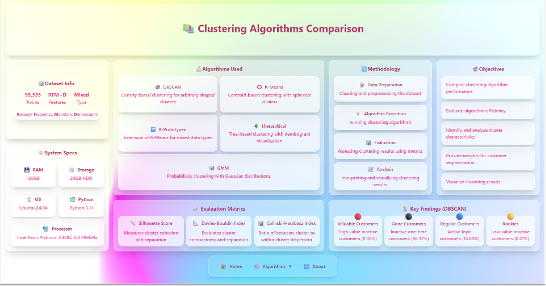
\includegraphics[width=12cm]{home}
        \end{center}
        Menampilkan ringkasan dari penelitian yang telah dilakukan.
        \item \textbf{Algorithms} \\
        \begin{center}
            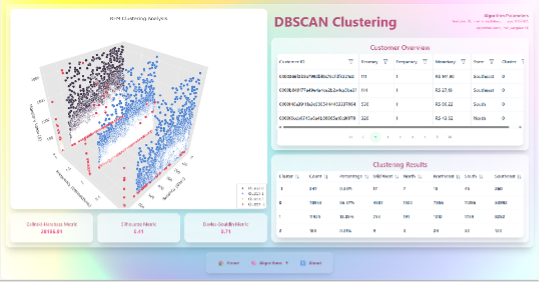
\includegraphics[width=12cm]{algorithms}
        \end{center}
        Menampilkan informasi terkait hasil \textit{clustering }dari suatu algoritma yang pengguna pilih.
        Ada lima komponen utama dalam
        tampilan ini, yaitu 3D \textit{Scatter Plot }yang menampilkan distribusi \textit{cluster }secara interaktif,
        karena setiap titik pada\textit{ plot }ini dapat dilihat informasi ringkasnya saat di \textit{hover}, \textit{plot }ini juga
        dapat di filter berdasarkan \textit{cluster} dengan menekan \textit{cluster }yang ingin disembunyikan pada
        \textit{legend }di bawah kanan \textit{plot}. \\
        Tampilan ini juga menampilkan daftar pelanggan\textit{ }pada tabel yang dilengkapi fitur
        \textit{searching}, \textit{sorting}, dan juga \textit{filtering}. Selain itu, terdapat tabel hasil \textit{clustering }yang berisi
        distribusi \textit{cluster }dengan distribusi geografis masing-masing \textit{cluster}. Kemudian, tampilan ini
        juga menampilkan parameter dan hasil metrik evaluasi dari algoritma yang dipilih.
        \item \textbf{About} \\
        \begin{center}
            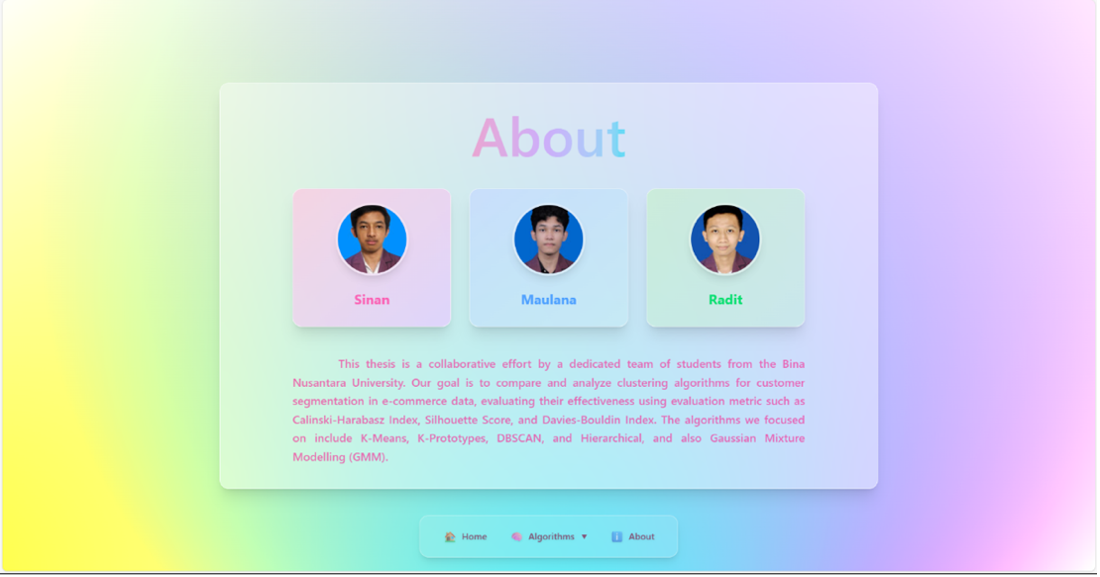
\includegraphics[width=12cm]{about}
        \end{center}
        Menampilkan daftar peneliti yang terlibat dalam penelitian ini, serta ringkasan tentang penelitian yang dilakukan.
    \end{itemize}


    \section{Backend Clustering (be-clustering)}
    Bagian ini menjelaskan cara instalasi dan menjalankan backend API yang dibangun menggunakan FastAPI dan PostgreSQL.

    \subsection{Instalasi secara \textit{Native}}

    \subsubsection{\textit{Requirements}}
    \begin{itemize}
        \item Python 3.11
        \item pip
        \item PostgreSQL (akses database)
    \end{itemize}

    \subsubsection{Langkah-langkah Instalasi}
    \begin{enumerate}
        \item \textbf{Clone repositori backend}

        \begin{mdframed}[style=codestyle]
            \small\texttt{git clone https://github.com/pt-sinan-akbar/be-clustering.git} \\
            \small\texttt{cd be-clustering}
        \end{mdframed}

        \item \textbf{Buat dan aktifkan virtual environment}

        \begin{mdframed}[style=codestyle]
            \small\texttt{python -m venv venv} \\
            \small\texttt{source venv/bin/activate}
        \end{mdframed}

        \item \textbf{Instal dependensi}

        \inlinecode{pip install -r requirements.txt}

        \item \textbf{Konfigurasi environment}

        \inlinecode{cp .env\_dummy .env}

        Edit file \texttt{.env} dan sesuaikan kredensial database PostgreSQL Anda.

        \item \textbf{Jalankan aplikasi}

        \inlinecode{uvicorn main:app --reload}

        API akan berjalan di \url{http://localhost:8080}
    \end{enumerate}

    \subsection{Instalasi dan Menjalankan menggunakan Docker}

    \subsubsection{\textit{Requirements}}
    \begin{itemize}
        \item Docker 28.x atau lebih baru, terinstal dan sedang berjalan.
    \end{itemize}

    \subsubsection{Langkah-langkah}
    Selain menggunakan metode instalasi ini, anda juga dapat \textit{pull} image yang telah disediakan di Docker Hub dengan perintah:

    \inlinecode{docker pull dta32/be-clustering:latest}
    Jika menggunakan metode \textit{pull} image, anda dapat langsung melompat ke langkah 4.
    \begin{enumerate}
        \item \textbf{Clone repositori backend}

        \begin{mdframed}[style=codestyle]
            \small\texttt{git clone https://github.com/pt-sinan-akbar/be-clustering.git} \\
            \small\texttt{cd be-clustering}
        \end{mdframed}

        \item \textbf{Salin dan edit file environment}

        \inlinecode{cp .env\_dummy .env}

        Edit file \texttt{.env} dan sesuaikan kredensial database PostgreSQL Anda.

        \item \textbf{Build Docker image}

        \inlinecode{docker build -t be-clustering:latest .}

        \item \textbf{Jalankan Docker container} \\
        Setelah image berhasil dibuat, jalankan sebagai sebuah kontainer dengan perintah berikut.

        \begin{mdframed}[style=codestyle]
            \small\texttt{docker run --name be-clustering-container} \\
            \small\texttt{-v \$(pwd)/.env:/app/.env -d -p 8080:8080 be-clustering:latest}
        \end{mdframed}

        Atau gunakan perintah berikut jika anda menggunakan metode \textit{pull} image.

        \begin{mdframed}[style=codestyle]
            \small\texttt{docker run --name be-clustering-container} \\
            \small\texttt{-v \$(pwd)/.env:/app/.env -d -p 8080:8080 dta32/be-clustering:latest}
        \end{mdframed}

        \item \textbf{Akses API}
        \url{http://localhost:8080}
    \end{enumerate}

    \subsubsection{Menghentikan dan Menghapus Kontainer}
    Untuk menghentikan kontainer:

    \inlinecode{docker stop be-clustering-container}
    Untuk menghapus kontainer setelah dihentikan:

    \inlinecode{docker rm be-clustering-container}

    \subsection{Prosedur Penggunaan Backend}
    Setelah aplikasi backend berhasil di-install dan dijalankan, backend dapat digunakan dengan menggunakan Frontend
    secara bersamaan, hal ini dikarenakan Backend hanya berguna untuk mengambil dan mengolah lalu menyajikan data
    yang diperlukan oleh Frontend.

\end{document}